\subsection{Coordinate Systems}

This section introduces the used coordinates systems and naming conventions that model the sensory system commonly used in computer vision.
Additionally, homogeneous coordinates allow efficient computation of rotation and translation with one matrix-vector multiplication and knowledge of it is a prerequisite.
Both~\cite{hartley_2004} and~\cite{corke_2011} provide excellent coverage of these topics.

\subsubsection*{Naming Conventions}

A point in space is referenced by a vector in that space.
The global reference frame is arbitrarily choosen in \emph{world coordinates}.
Within that world coordinate system exist one or more sensors spanning their own coordinate system.
Referencing the point relative to such a sensor yields \emph{camera coordinates}.
The sensor itself performs some form of dimension reducing projection of the three dimensional point to a two dimensional point, an \emph{image coordinate}.
\emph{Image coordinates} are an intermediate representation before discretizing the point to individual pixels, called \emph{pixel coordinates}.
Inverting this projection results in \emph{spherical coordinates}, camera coordinates with unit length that just encode the direction of a light ray that hits a pixel.
Different sensor models describe these projecting transformations mathematically.
Note, that the relative transformation between \emph{camera coordiantes} and \emph{world coordinates}, the sensors \emph{pose}, can change over time.
Multiple sensors can exist within the \emph{world coordinate system}.

\subsubsection*{Coordinate Transformations and Pose}

\begin{figure}[H]
    \scalebox{0.8}{%
    \tikzset{every picture/.style={line width=0.75pt}} %set default line width to 0.75pt        

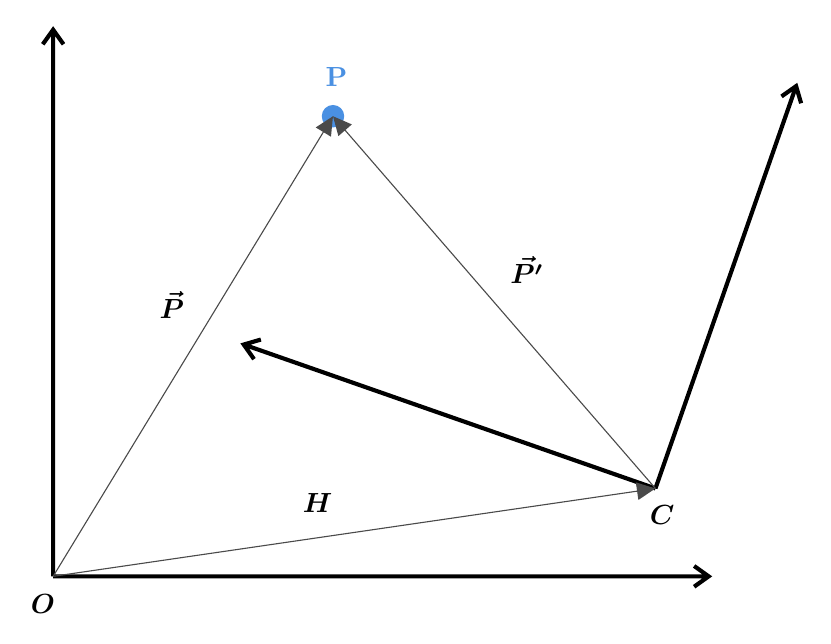
\begin{tikzpicture}[x=0.75pt,y=0.75pt,yscale=-1,xscale=1, style={font=\boldmath}]
%uncomment if require: \path (0,300); %set diagram left start at 0, and has height of 300

%Shape: Circle [id:dp39370051291999986] 
\draw  [draw opacity=0][fill={rgb, 255:red, 74; green, 144; blue, 226 }  ,fill opacity=1 ] (152.42,50.67) .. controls (152.42,47.68) and (154.84,45.25) .. (157.83,45.25) .. controls (160.82,45.25) and (163.25,47.68) .. (163.25,50.67) .. controls (163.25,53.66) and (160.82,56.08) .. (157.83,56.08) .. controls (154.84,56.08) and (152.42,53.66) .. (152.42,50.67) -- cycle ;
%Shape: Axis 2D [id:dp7479977699053467] 
\draw [line width=1.5]  (23,272.35) -- (338.83,272.35)(23,9) -- (23,272.35) -- cycle (331.83,267.35) -- (338.83,272.35) -- (331.83,277.35) (18,16) -- (23,9) -- (28,16)  ;
%Shape: Axis 2D [id:dp43513516367104466] 
\draw [line width=1.5]  (313.19,230.01) -- (380.96,36.17)(114.83,160.67) -- (313.19,230.01) -- cycle (373.93,41.13) -- (380.96,36.17) -- (383.37,44.43) (119.79,167.7) -- (114.83,160.67) -- (123.09,158.26)  ;
%Straight Lines [id:da8557794245884446] 
\draw [color={rgb, 255:red, 74; green, 74; blue, 74 }  ,draw opacity=1 ]   (23,272.35) -- (156.27,53.23) ;
\draw [shift={(157.83,50.67)}, rotate = 481.31] [fill={rgb, 255:red, 74; green, 74; blue, 74 }  ,fill opacity=1 ][line width=0.08]  [draw opacity=0] (8.93,-4.29) -- (0,0) -- (8.93,4.29) -- cycle    ;
%Straight Lines [id:da7386423573093532] 
\draw [color={rgb, 255:red, 74; green, 74; blue, 74 }  ,draw opacity=1 ]   (23,272.35) -- (310.22,230.45) ;
\draw [shift={(313.19,230.01)}, rotate = 531.7] [fill={rgb, 255:red, 74; green, 74; blue, 74 }  ,fill opacity=1 ][line width=0.08]  [draw opacity=0] (8.93,-4.29) -- (0,0) -- (8.93,4.29) -- cycle    ;
%Straight Lines [id:da6638828901158511] 
\draw [color={rgb, 255:red, 74; green, 74; blue, 74 }  ,draw opacity=1 ]   (313.19,230.01) -- (159.8,52.93) ;
\draw [shift={(157.83,50.67)}, rotate = 409.1] [fill={rgb, 255:red, 74; green, 74; blue, 74 }  ,fill opacity=1 ][line width=0.08]  [draw opacity=0] (8.93,-4.29) -- (0,0) -- (8.93,4.29) -- cycle    ;

% Text Node
\draw (153,26) node [anchor=north west][inner sep=0.75pt]  [color={rgb, 255:red, 74; green, 144; blue, 226 }  ,opacity=1 ] [align=left] {$\displaystyle \mathbf{P}$};
% Text Node
\draw (73,134) node [anchor=north west][inner sep=0.75pt]   [align=left] {$\displaystyle \vec{P}$};
% Text Node
\draw (11,280) node [anchor=north west][inner sep=0.75pt]   [align=left] {$\displaystyle O$};
% Text Node
\draw (309.19,237.01) node [anchor=north west][inner sep=0.75pt]   [align=left] {$\displaystyle C$};
% Text Node
\draw (242,117) node [anchor=north west][inner sep=0.75pt]   [align=left] {$\displaystyle \vec{P'}$};
% Text Node
\draw (142,231) node [anchor=north west][inner sep=0.75pt]   [align=left] {$\displaystyle H$};


\end{tikzpicture}

    }
    \caption[Coordinate Transformation]{Relationship between different representation of the same point in different coordinate systems. The relationship displayed here and the corresponding linear algebra holds true for cartesian coordinate systems of any dimension.}
\end{figure}

Let $\mathbf{O}$ be the origin of the \emph{world coordinate system}.
A three dimensional vector $\vec{P} = \rowvecxxx{U}{V}{W}$ represents a point in this room relative to the origin $\mathbf{O}$.
Seeing this point $\mathbf{P}$ from a camera $\mathbf{C}$ within the same room is equivalent to changing the coordinate system from \emph{world coordinates} to \emph{camera coordinates} of that sensor.
The relative rotation and translation of the camera $\mathbf{C}$ to the room is also called its \emph{pose}.
It is parametrized by a rotation matrix $R$ and a translation vector $\vec{t}$.
Homogeneous coordinates provide a computational more efficient way to apply the transformation to vectors by $4 \times 4$ matrix-vector multiplication instead of $3 \times 3$ matrix-vector multiplication and an additional $3 \times 1$ vector addition.
The point $\mathbf{P}$ seen from the camera $\mathbf{C}$ is computed with the homogeneous transformation matrix $H = \begin{bmatrix} R & \vec{t} \\ 
    \begin{matrix}0 & 0 & 0\end{matrix} & 1 \end{bmatrix}$.
\begin{equation}
\begin{aligned}
    \colvech{X}{Y}{Z}&= \begin{pmatrix}
        r_{11} & r_{12} & r_{13} & t_x \\
        r_{21} & r_{22} & r_{23} & t_y \\
        r_{31} & r_{32} & r_{33} & t_z \\
        0      & 0      & 0      & 1 \\
    \end{pmatrix} \colvech{U}{V}{W} \\
    \vec{P}' &= H \vec{P}
\end{aligned}
\end{equation}

Coordinate transformations do not loose information.
